\subsection{Maxwell equations}

\fcolorbox{red}{white}{

	\begin{tabularx}{\columnwidth}{llX}
		Name & Differential equations & meaning \\
		Gauss's law & $\nabla \cdot \mathbf{E} = \frac {\rho} {\varepsilon_0}$ &  The electric field in a volume is proportional to the charge inside.\\
		Gauss's law for magnetism & $\nabla \cdot \mathbf{B} = 0$ & There are no magnetic monopoles. All magnetic field lines are closed loops \\
		Induction equation & $\nabla \times \mathbf{E} = -\frac{\partial \mathbf{B}} {\partial t}$ & The voltage accumulated around a closed circuit is proportional to the time rate of change of the magnetic flux it encloses.\\
		Ampère's circuital law & $\nabla \times \mathbf{B} = \mu_0\left(\mathbf{J} + \varepsilon_0 \frac{\partial \mathbf{E}} {\partial t} \right) $& Electric currents and changes in electric fields are proportional to the magnetic field circulating about the area they pierce.\\
	\end{tabularx}
}

\subsection{Electrostatics}
	
	A direct concequence of Ampère's circuit law states the conservation of charge 
	$$  \nabla \cdot \mathbf{J} = - {\partial \rho \over \partial t} $$
	
	\renewcommand{\arraystretch}{2}
	\begin{tabularx}{\columnwidth} {lXX}
		\hline
		&point charge & distribiuted \\
		\hline
		Coulomb force&
		$\mathbf{F} = \dfrac{Q}{4\pi \varepsilon_0}\cdot \sum\limits_{i} q_i \dfrac{\mathbf{r_i}}{r_i^3}$&
		$\mathbf{F}(\textcolor{red}{\mathbf{r}}) = \dfrac{Q}{ 4\pi\varepsilon_0}\int\rho(\textcolor{darkgreen}{\mathbf{r'}}) \dfrac{\textcolor{red}{\mathbf{r}} - \textcolor{darkgreen}{\mathbf{r'}}}{|\textcolor{red}{\mathbf{r}} - \textcolor{darkgreen}{\mathbf{r'}}|^3} dV$ \\
		\hline
		Electrical Field&
		 $ \mathbf{E} = \dfrac{\mathbf{F}}{Q} = \sum\limits_i\dfrac{q_i}{4\pi\epsilon_0}\dfrac{\mathbf{r - r_i}}{|r-r_i|^3}$ &
		 $ \mathbf{E}(\textcolor{red}{\mathbf{r}}) =  \dfrac{1}{4\pi\varepsilon_0} \int \rho(\textcolor{darkgreen}{\mathbf{r'}}) \dfrac{\textcolor{red}{\mathbf{r}} - \textcolor{darkgreen}{\mathbf{r'}}}{|\textcolor{red}{\mathbf{r}} - \textcolor{darkgreen}{\mathbf{r'}}|^3}dV$ \\
		 & &  $\nabla\times\mathbf{E} = 0 \Rightarrow$ potential field $\mathbf{E}=-\nabla \varphi$\\
		\hline 
		Potential &
		$\varphi(\mathbf{r}) = \sum\limits_i \dfrac{ q_i}{4\pi\epsilon_0 |\mathbf{r}-\mathbf{r_i|}}$&
		$\varphi(r_1, r_2) = \int\limits_{r_1}^{r_2} \mathbf{E}\cdot d\mathbf{l}$\\
		\hline 
		Electric Flux & &
		$\mathbf{\Phi} = \int\limits_S \mathbf{E}\cdot\mathbf{n} dA$
		\\
		\hline 
		&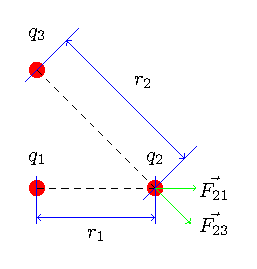
\includegraphics[scale = 1]{tikz/pointcharge.pdf} & 		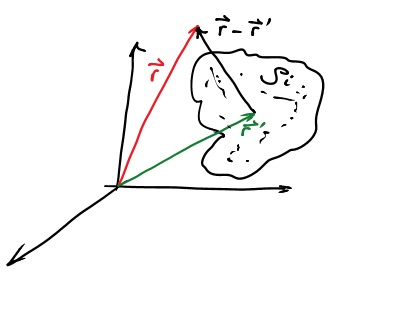
\includegraphics[width = 4cm]{images/elfield} \\
		\hline 
		Dipole formulas & $\varphi(\mathbf{r}) = \dfrac{1}{4\pi\epsilon_0}\dfrac{\mathbf{pr}}{r^3}$&
		$\mathbf{E}(\mathbf{r}) = \dfrac{1}{4\pi\epsilon_0r^3}(3\mathbf{(p\hat{r})\hat{r}-p)}$\\
		\hline 
	\end{tabularx}

	\renewcommand{\arraystretch}{1.2}

	\subsection{Electrical field in Matter}
		\begin{tabularx}{\columnwidth}{lXX}
			polarisation & $\mathbf{p} \propto \mathbf{E}$ & $p_i = \alpha_{ij}E_j$\\
			Dipole moment & $\mathbf{P} = \epsilon_0 x_{ij} E_j$ &\\
			Electrical displacement & $\mathbf{D} = \epsilon_0\mathbf{E} + \mathbf{P} = \epsilon_0 (1+\chi)\mathbf{E} = \epsilon_0\epsilon_r\mathbf{E}$&
			$D = \epsilon_0\epsilon_{ij}E_j$\\
			
		\end{tabularx}

	\subsection{Energy in the electrical field}
		{\def \arraystretch{2}	
	\begin{tabularx}{\columnwidth}{lllXX}
		&capacity & charge & work&energy density\\
		General & $C = \dfrac{Q}{U}$ & $Q = \oint\mathbf{E}d\sigma$ & $W = \int U dQ$& $w_{el} = \dfrac{W}{V}$\\
		Plate capacitor & $C = \epsilon_0\dfrac{A}{d}$ & &$W = \frac{1}{2}CU^2 = \frac{1}{2}\epsilon_0 \mathbf{E}^2A d $ & $w_{el}= \frac{1}{2}\epsilon_0\epsilon_{ij}\mathbf{E_j E_i}= \frac{1}{2}\mathbf{D_i E_i}$\\

		
	\end{tabularx}
	
		The permittivity tensor has to be symmetric: 
		$$
		\epsilon_{ij} = \begin{bmatrix}
		\epsilon_1 & 0 & 0 \\ 0 & \epsilon_2 & 0 \\ 0 & 0 & \epsilon_3 \\
		\end{bmatrix}
		$$ 

		\subsection{Magnetostatics}

		\begin{tabularx}{\columnwidth}{p{3cm}X}
		Strom       & $I = \dfrac{dQ}{dt} = \iint\limits_\epsilon \bm j d\bm A \qquad $ Stromdichte $j = \dfrac{I}{A}$\\
			
		Biot Savart & $\vec B = \dfrac{\mu_0}{4\pi}\cdot I \int \dfrac{ds\times \mathbf{r}}{r^3} = $
		$\dfrac{\mu_0}{4\pi}\iiint \bm j(\bm r') \times \dfrac{\bm r - \bm r'}{|\bm r - \bm r'|^3}dV$ \\
		flux conservation & $\nabla\cdot \mathbf{B} = 0$ all  magnetic field lines are closed\\
		Ampère law	& $\nabla\times \mathbf{B} = \mu_0 \mathbf{j}$\\
		Ohm's law			&$\bm j = \sigma \bm E\qquad \bm E =  \rho \bm j$\\
					 
		Lorentz force: point charge & $\mathbf{F} = q(\mathbf{E+v\times B})	$\\
		Lorentz force: wire  & $\bm F = I\cdot \bm l \times \bm B$\\
		
		Magnetic Moment& $\bm M = \bm m  \times \bm B \qquad  M = m  B \cdot \sin\alpha \qquad m = I A\cdot \bm n$\\
 		\end{tabularx}
	}
		\subsection{Magnetic field in Matter}
		\begin{tabularx}{\columnwidth}{lX}
			Magnetized Field & $  \mathbf{B} = \mu_0(1+ \chi_m)\mathbf{H} =  \mu_0\mu_r\mathbf{H}$	\\
		\end{tabularx}
		
		\subsection{Energy in magnetic field}
		\begin{tabularx}{\columnwidth}{lX}
			$w_{mag} = \frac{1}{2}\mathbf{BH}= \frac{1}{2}\mu_0\mu_{ij}H_j H_i$\\
		\end{tabularx}

				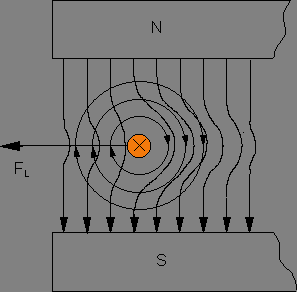
\includegraphics[scale=0.5]{images/DrahtZwischenPolen.png}
				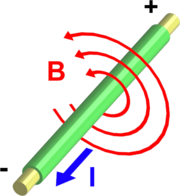
\includegraphics[scale=0.5]{images/B-Feld.png}
			$ \vec{p}=q\cdot\vec{d} $
			$ I = \sigma_{11} \cdot E_1 \cdot A $
		$ R=\rho\cdot\frac{l}{A}=\frac{1}{\sigma} \cdot\frac{l}{A}$\\

		\begin{tabular}{|c|c|}
				\hline Strom & Daumen \\ 
				\hline B-Feld & Zeigefinger \\ 
				\hline Kraft & Mittelfinger \\ 				
				\hline
			\end{tabular} 
			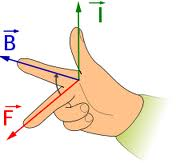
\includegraphics[scale=0.5]{images/handregel.jpg}	
			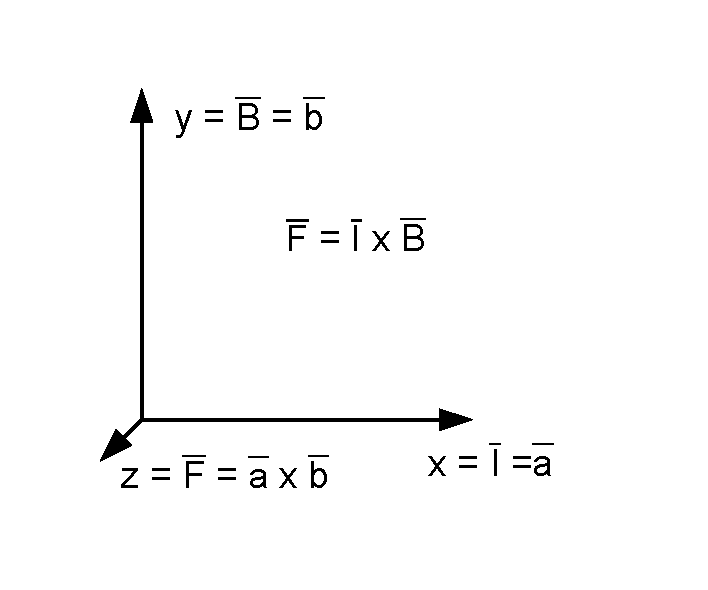
\includegraphics[scale=0.5]{images/kreuzprodukt.pdf}
